\documentclass{article}%
\usepackage[T1]{fontenc}%
\usepackage[utf8]{inputenc}%
\usepackage{lmodern}%
\usepackage{textcomp}%
\usepackage{lastpage}%
\usepackage[head=40pt,margin=0.5in,bottom=0.6in]{geometry}%
\usepackage{graphicx}%
%
\title{\textbf{Sebin intentó allanar la residencia de Saverio Vivas en Catia}}%
\author{El Nacional Web}%
\date{19/10/2018}%
%
\begin{document}%
\normalsize%
\maketitle%
\textbf{URL: }%
http://www.el{-}nacional.com/noticias/politica/sebin{-}intento{-}allanar{-}residencia{-}saverio{-}vivas{-}catia\_256442\newline%
%
\textbf{Periodico: }%
EN, %
ID: %
256442, %
Seccion: %
Política\newline%
%
\textbf{Palabras Claves: }%
Política, Sebin, Diosdado Cabello, Caracas\newline%
%
\textbf{Derecho: }%
1.3%
, Otros Derechos: %
NO\_TIENE%
, Sub Derechos: %
1.3.4%
\newline%
%
\textbf{EP: }%
NO\newline%
\newline%
%
\textbf{\textit{El activista forma parte del Movimiento por la Democracia e Inclusión~}}%
\newline%
\newline%
%
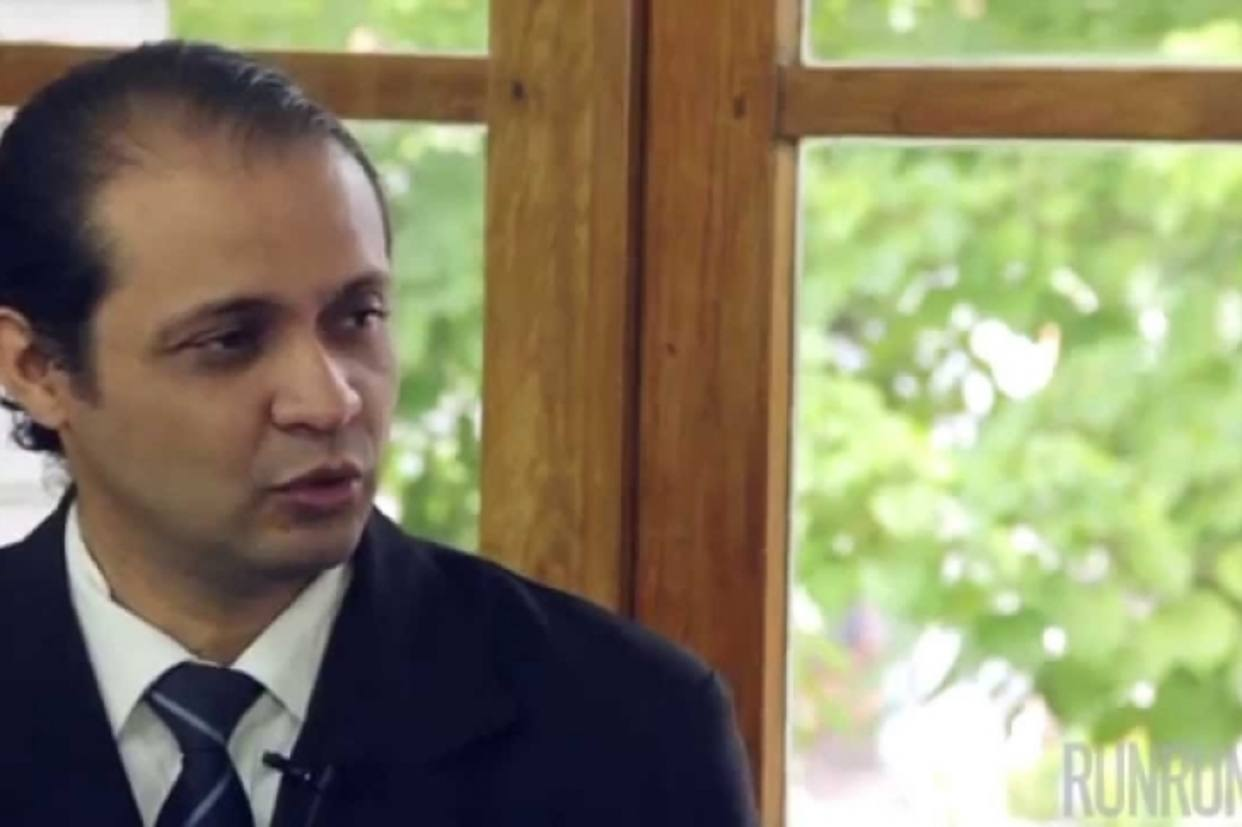
\includegraphics[width=300px]{175.jpg}%
\newline%
%
Nicmer Evans, vocero del Movimiento por la Democracia y la Inclusión (MDI), denunció que funcionarios del Servicio Bolivariano de Inteligencia Nacional (Sebin)~intentaron allanar la vivienda de Saverio Vivas, directivo del MDI.%
\newline%
%
“Nos informan que en este momento funcionarios de Sebin intentan entrar a la vivienda de Saverio Vivas en Catia”, escribió Evans en su Twitter.%
\newline%
%
Hasler Iglesias, dirigente juvenil de Voluntad Popular, indicó que Vivas fue “amenazado” por Diosdado Cabello, presidente de la asamblea nacional constituyente.%
\newline%
%
“Denunciamos la persecución contra Vivas, líder social de Catia durante años, y quien ha participado activamente en la Plataforma de Conflicto. Diosdado Cabello lo amenaza por VTV, y de inmediato el SEBIN allana su residencia. ¡Basta ya!”, comentó Iglesias.%
\newline%
%
Asimismo, el partido político La Causa R indicó que el gobierno se “ensaña” contra Vivas.%
\newline%
%
“La ola represiva de la dictadura se ensaña en este momento contra Vivas, compañero de lucha en la Plataforma De Conflicto. Repudiamos esta escalada terrorista del régimen de Maduro”, señaló el partido.%
\newline%
%
\end{document}